\documentclass[12pt,a4paper]{article}
\usepackage[utf8]{inputenc}
\usepackage{amsmath}
\usepackage{amsfonts}
\usepackage{amssymb}
\usepackage{graphicx}
\author{José Antonio García Hernández}
\title{2-Flavor Lattice QCD}

\usepackage{tikz}
\usetikzlibrary{decorations.markings}
\usetikzlibrary{math} %needed tikz library
\usetikzlibrary{arrows}
\newcommand*{\eps}{0.05}
\usepackage{subcaption}

\usepackage{dsfont}

\newcommand{\tr}{\text{Tr}\,}
\newcommand{\re}{\text{Re}\,}
\newcommand{\SU}[1]{\text{SU}({#1})}

\newcommand{\su}[1]{\mathfrak{su}({#1})}

\usepackage{url}

\begin{document}
\maketitle

\section{SU($N$) gauge theory}

    An element of a group \SU{$N$} is represented by 
    \begin{equation}
        U = e^{A} \in \SU{N}
    \end{equation}
where $A\in\su{N}$ is traceless and anti-Hermitian, an element of the Lie algebra. There are $N^2-1$ generators $T^a$ of the algebra, and they satisfy

    \begin{equation}
       \tr T = 0, \ \ \ T^{\dagger} = -T, \ \ \ \tr [T^aT^b] = -\frac{1}{2}\delta^{ab}.
    \end{equation}
    Any element of the algebra can be written as
    \begin{equation}
        A = A^aT^a , \ \ \ A^a \in \mathbb{R},
    \end{equation}
    sum over repeated indices assumed.

    
    
    
    We study the 4-dimensional SU(3) lattice gauge theory with the compact formulation. In this formulation we consider compact link variables $U_{x,\mu}\in \text{SU}(3)$ rather than the Lie algebra-valued fields $A_{x,\mu}$. The compact variables $U_{x,\mu}$ become the fundamental fields to be integrated over the functional integral. One great advantage of the compact formulation is that we no longer require to fix the gauge.

Link variables are oriented, so they naturally live in the links between neighboring points on the lattice. Thus, the variable $U_{x,\mu}$ is defined in the link between points $x$ and $x + \hat \mu$ in the positive $\mu$ direction, see Fig.\ \ref{fig:link}. We define the variable between points $x$ and $x + \hat \mu$ pointing in the negative direction via
\begin{equation}
	U_{x+\hat\mu,-\mu} \equiv  U^{\dagger}_{x,\mu}, 
\end{equation}
see Fig.\ \ref{fig:conjg_link}.


\begin{figure}
\begin{center}
\begin{subfigure}{0.45\textwidth}
	\begin{center}
	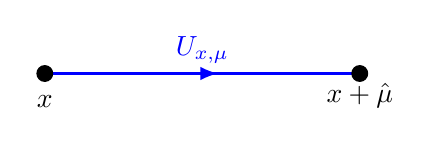
\begin{tikzpicture}
		\tikzset{middlearrow/.style={decoration={markings,mark= at position 0.55 with {\arrow{#1}} ,},postaction={decorate}}};
		\draw[middlearrow={latex}, very thick,blue] (0,0)--(4,0);
		\draw[blue] (2,0) node[above] {$U_{x,\mu}$};
		\filldraw[black] (0,0) circle(0.1);
		\draw (0,-0.35) node[]{$x$};
		\filldraw[black] (4,0) circle(0.1) node[below]{$x+\hat{\mu}$};
	\end{tikzpicture}
	\end{center}
	\caption{Link variable at point $x$ in the $\mu$ direction.}
	\label{fig:link}
\end{subfigure}
\begin{subfigure}{0.45\textwidth}
	\begin{center}
	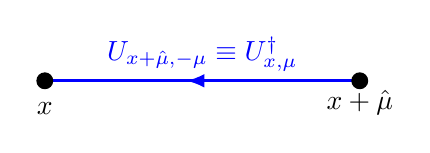
\begin{tikzpicture}
		\tikzset{middlearrow/.style={decoration={markings,mark= at position 0.55 with {\arrow{#1}} ,},postaction={decorate}}};
		\draw[middlearrow={latex}, very thick,blue] (4,0)--(0,0);
		\draw[blue] (2,0) node[above] {$  U_{x+\hat\mu,-\mu} \equiv  U^{\dagger}_{x,\mu}$};
		\filldraw[black] (0,0) circle(0.1);
		\draw (0,-0.35) node[]{$x$};
		\filldraw[black] (4,0) circle(0.1) node[below]{$x+\hat{\mu}$};
	\end{tikzpicture}
	\end{center}
	\caption{Link variable at point $x+\hat\mu$ in the $-\mu$ direction.}
	\label{fig:conjg_link}
\end{subfigure}
\end{center}
\caption{Graphical representation of link variables.}
\end{figure}

\begin{figure}
\centering
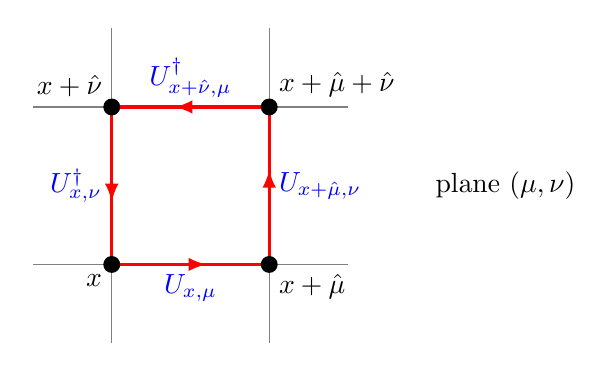
\begin{tikzpicture}
		\tikzset{middlearrow/.style={decoration={markings,mark= at position 0.6 with {\arrow{#1}} ,},postaction={decorate}}};
		\draw[step=2cm,color=gray] (-1,-1) grid (3,3);
		\draw[middlearrow={latex}, very thick,red] (0,0) --(2,0);
		\draw[middlearrow={latex}, very thick,red] (2,0)--(2,2);
		\draw[middlearrow={latex}, very thick,red] (2,2)--(0,2);
		\draw[middlearrow={latex}, very thick,red] (0,2)--(0,0);
		\filldraw[black] (0,0) circle(0.1);
		\filldraw[black] (2,0) circle(0.1);
		\filldraw[black] (2,2) circle(0.1);
		\filldraw[black] (0,2) circle(0.1);
		\draw[] (0,0) node[below left] {$x$};
		\draw[] (2,0) node[below right] {$x+\hat\mu$};
		\draw[] (0,2) node[above left] {$x+\hat\nu$};
		\draw[] (2,2) node[above right] {$x+\hat\mu+\hat\nu$};
		
		\draw[] (5,1) node[] {plane $(\mu,\nu$)};
		
		\draw[blue] (1,0) node[below] {$U_{x,\mu}$};
		\draw[blue] (2,1) node[right] {$U_{x+\hat\mu,\nu}$};	
		\draw[blue] (1,2) node[above] {$U^{\dagger}_{x+\hat\nu,\mu}$};
		\draw[blue] (0,1) node[left] {$U^{\dagger}_{x,\nu}$};
			
	\end{tikzpicture}
	\caption{Plaquette $U_{x,\mu\nu}$.}
\end{figure}

Under a gauge transformation the link variables transform as
\begin{equation}
	U'_{x,\mu} = \Omega_x U_{x,\mu} \Omega_{x+\hat\mu}^{\dagger},
\end{equation}
where $\Omega_x\in\text{SU}(3)$. We refer to \cite{gattringer} for a complete discussion on lattice gauge theory.

\subsection{Action}
For SU($N$), the lattice gauge action reads
\begin{equation}
	\label{eq:wilson_action}
	S_G[U] = \frac{\beta}{N}\sum_x \sum_{\mu < \nu} \text{Re}\ \text{Tr} \left[\mathds{1} - U_{x,\mu\nu} \right],
\end{equation}
where $\beta = \frac{2N}{g^2}$. The plaquettes are defined by
\begin{equation}
	\label{eq:plaquette}
	U_{x,\mu\nu} = U_{x;\mu,\nu} = U_{x,\mu}U_{x+\hat{\mu},\nu}U_{x+\hat{\nu},\mu}^{\dagger}U_{x,\nu}^{\dagger} 
\end{equation}

Sum of plaquette variables
\begin{equation}
	\label{eq:Sp}
	S_{\text{P}} = \frac{1}{N} \sum_x\sum_{\mu < \nu} \text{Re}\ \text{Tr} [U_{\mu\nu}(x)]
\end{equation}
we define
\begin{equation}
	\label{eq:Ep}
	E_{\text{P}} =\frac{ \langle S_{\text{P}} \rangle}{D V}
\end{equation}
where $V$ is the volume of the lattice and $D = \frac{d(d-1)}{2}$ is the number of planes of rotation.

Staples
\begin{equation}
	\label{eq:staples}
	\Sigma_{x,\mu} = \sum_{\nu \neq \mu} \left[ U_{x,\nu}U_{x+\hat{\nu},\mu}U_{x+\hat{\mu},\nu}^{\dagger} + U_{x-\hat{\nu},\nu}^{\dagger}U_{x-\hat{\nu},\mu}U_{x+\hat{\mu}-\hat{\nu},\nu}\right]
\end{equation}

The change in the action  by a local update when changing $U_{x,\mu} \to U'_{x,\mu}$ is
\begin{equation}
	\label{eq:DS}
	\Delta S = -\frac{\beta}{N} \text{Re } \text{Tr} \left[ \left( U'_{x,\mu} - U_{x,\mu} \right)\Sigma_{x,\mu}^{\dagger}\right]
\end{equation}

In SU(3) the SU(2) elements are of the form
\begin{equation}
\label{eq:SU2_subgroups}
	R = \begin{pmatrix}
		r_{11} & r_{12} & 0 \\
		r_{21} & r_{22} & 0 \\
		0      & 0      & 1 
	\end{pmatrix},\ S = \begin{pmatrix}
		s_{11} & 0 & s_{12} \\
		0      & 1 & 0 \\
		s_{21} & 0 & s_{22} 
	\end{pmatrix},\ T = \begin{pmatrix}
		1 & 0 & 0 \\
		0 & t_{11} & t_{12} \\
		0 & t_{21} & t_{22}
	\end{pmatrix}.
\end{equation}

\begin{figure}
\centering
\begin{tikzpicture}[scale=2]    
\tikzset{middlearrow/.style={decoration={markings,mark= at position 0.6 with {\arrow{#1}} ,},postaction={decorate}}};
   
    \draw[white] (-\eps,-1-\eps) rectangle (1+\eps,1+\eps);
    \draw[middlearrow={latex}] (0,\eps) -- (0,1);
    \draw[middlearrow={latex}] (0,1) -- (1,1);
    \draw[middlearrow={latex}] (1,1) -- (1,\eps);
    
    \draw[middlearrow={latex}] (0,-\eps) -- (0,-1);
    \draw[middlearrow={latex}] (0,-1) -- (1,-1);
    \draw[middlearrow={latex}] (1,-1) -- (1,-\eps);
    
    
    \draw[blue, very thick,-latex] (0,0) -- (1,0);
    \draw (0.5,0) node[above] {$U_{x,\mu}$};
   
    \draw[-latex] (2.5,0)--(3,0) node[above]{$\hat\mu$};
    \draw[-latex] (2.5,0)--(2.5,0.5) node[right]{$\hat\nu$};
\end{tikzpicture}
\caption{Sum of staples $\Sigma_{x,\mu}$.}
\end{figure}

\subsection{Field strength tensor}

We can define the field strengh tensor on the lattice with either the \emph{Plaquette} or \emph{Clover} definition. A clover is defined as follows
\begin{eqnarray}
    Q_{x,\mu\nu} & = & U_{x,\mu}U_{x+\hat{\mu},\nu}U_{x+\hat{\nu},\mu}^{\dagger}U_{x,\nu}^{\dagger}  +  \nonumber\\
    & & U_{x,\nu}U_{x-\hat{\mu}+\hat{\nu},\mu}^{\dagger}U_{x-\hat{\mu},\nu}^{\dagger}U_{x-\hat{\mu},\mu}  + \nonumber\\ 
    & & U_{x-\hat{\mu},\mu}^{\dagger}U_{x-\hat{\mu}-\hat{\nu},\nu}^{\dagger}U_{x-\hat{\mu}-\hat{\nu},\mu}U_{x-\hat{\nu},\nu}+\nonumber\\
    &  & U_{x-\hat{\nu},\nu}^{\dagger} U_{x-\hat{\nu},\mu}U_{x+\hat{\mu}-\hat{\nu},\nu}U_{x,\mu}^{\dagger}.
\end{eqnarray}

\tikzmath{\eps= 0.05; \ep = 0.08;}
 

\begin{figure}
\begin{center}
    \begin{tikzpicture}[decoration={markings,mark= at position 0.15 with {\arrow[scale=2,>=latex]{>}},markings,mark= at position 0.4 with {\arrow[scale=2,>=latex]{>}},mark= at position 0.65 with {\arrow[scale=2,>=latex]{>}},mark= at position 0.9 with {\arrow[scale=2,>=latex]{>}}},scale=2.3]
        \draw[postaction={decorate}]  (\eps + \ep,\eps)--(1-\eps,\eps)--(1-\eps,1-\eps)--(\eps,1-\eps)--(\eps, \ep + \eps);
        \draw[postaction={decorate}] (-\eps,\eps+\ep)--(-\eps,1-\eps)--(-1+\eps,1-\eps)--(-1+\eps,\eps)--(-\eps-\ep,\eps);
        \draw[postaction={decorate}] (-\eps-\ep,-\eps)--(-1+\eps,-\eps)--(-1+\eps,-1+\eps)--(-\eps,-1+\eps)--(-\eps,-\eps-\ep);
        \draw[postaction={decorate}] (\eps,-\eps-\ep)--(\eps,-1+\eps)--(1-\eps,-1+\eps)--(1-\eps,-\eps)--(\ep+\eps,-\eps); 
        
        %\fill[red] (0,0) circle(\eps);
        \fill (1,0) circle(\eps);
        \fill (1,1) circle(\eps);
        \fill (0,1) circle(\eps);
        \fill (-1,0) circle(\eps);
        \fill (0,-1) circle(\eps);
        \fill (-1,-1) circle(\eps);
        \fill (-1,1) circle(\eps);
        \fill (1,-1) circle(\eps);

        \draw (0,0) node[]{$x$};
        
        %\draw (0,-1.3) node[below]{$Q_{x,\mu\nu}$};
    \end{tikzpicture}
\end{center}    
\caption{A clover in the $(\mu\nu)$ plane is the sum of four oriented plaquettes $Q_{x;\mu,\nu} = U_{x;\mu,\nu} + U_{x;\nu,-\mu} + U_{x;-\mu,-\nu} + U_{x;-\nu,\mu}$ at some given point $x$.}
\end{figure}

Field strength tensor with the plaquette definition
\begin{equation}
    F^{\text{plaquette}}_{x,\mu\nu} = i(\mathds{1} - U_{x,\mu\nu}).
\end{equation}

Field strength tensor with the clover definition
\begin{equation}
    F^{\text{clover}}_{x,\mu\nu} = \frac{1}{8}\left[ Q_{x,\mu\nu} -  Q_{x,\mu\nu}^{\dagger}\right].
\end{equation}

\subsection{Energy density}
    
    In the continuum the definition of the energy density at $x$ is
    
    \begin{equation}
        E = \frac{1}{4} F_{\mu\nu}^{a}(x)F_{\mu\nu}^{a}(x) = -\frac{1}{2} \tr\left( F_{\mu\nu}(x)F_{\mu\nu}(x)\right),
    \end{equation}
where sum over repeated indices is assumed.
A possibility of defining the energy density on the lattice is by using the plaquette
\begin{equation}
    E = \frac{2}{V}\sum_{x,\mu<\nu}\re\tr\left(\mathds{1} - U_{x,\mu\nu} \right)
\end{equation}
or by using the more symmetric definition with the clover
\begin{eqnarray}
    E & = & -\frac{1}{2V}\sum_{x,\mu,\nu}\tr\left[F^{\text{clover}}_{\mu\nu}F^{\text{clover}}_{\mu\nu} \right]\\
      & = & -\frac{1}{64V}\sum_{x,\mu<\nu} \re\tr\left( Q_{x,\mu\nu} -  Q_{x,\mu\nu}^{\dagger}\right)^2
\end{eqnarray}




	\subsection{Polyakov Loop}
	The polyakov loop is defined as the product of the link variables in the Euclidean time direction over a closed loop
	\begin{equation}
		P_{\vec{x}} = \text{Tr}\,\prod_{t_\text{E}=1}^{L_t}U_{(\vec{x},t_\text{E}),4}.
	\end{equation}

\subsection{Static quark potential}
One important quantity involving Polyakov loops is their correlation. The correlation function of Polyakov loops is related to the static quark potential $V(r)$ as
\begin{equation}
	\left\langle P_{\vec{x}} P_{\vec{y}}^{\dagger} \right\rangle \propto e^{-L_t a V(r)} \left(1 +\mathcal{O}\left( e^{-L_t a \Delta E}\right) \right),
\end{equation}
where $r = |\vec{x} - \vec{y}\,|$. Numerically speaking, we compute

\begin{equation}
	\langle P_{\vec{x}} P_{\vec{y}}^{\dagger} \rangle = \frac{1}{3V}\sum_{x,\mu = 1,2,3}  P_{\vec{x}} P_{\vec{x}+r\hat{\mu}}^{\dagger}.
\end{equation}

 Up to a constant the static quark potential is
\begin{equation}
	aV(r) = - \log \left\langle P_{\vec{x}} P_{\vec{y}}^{\dagger} \right\rangle/L_t.
\end{equation}

We use the Cornell potential to parametrize $V(r)$
\begin{equation}
	V(r) = A + \frac{B}{r} + \sigma r,
\end{equation}
here $A$ is an irrelevant additive constant, $B$ is the Coulomb part of the potential and $\sigma$ is the so called \textit{string tension}.

\section{Setting physical scales}
One method of defining a physical scale is related to the static potential. First the Sommer parameter is defined as $r_0 \approx 0.5 \ \text{fm}$, is a physical length where, roguhly speaking, the potential becomes linear.

First we compute the force 
\begin{equation}
	\label{eq:force}
	-F(r) = \frac{dV(r)}{dr} = \sigma - \frac{B}{r^2}.
\end{equation}

Using experimental data for heavy quark-antiquark pairs ($\bar{b}b$ and $\bar{c}c$) it is found that 
\begin{equation}
	-F(r_0)r_0^2 = 1.65, \ \ \ \text{where} \ \ \ r_0 \simeq 0.5 \ \text{fm}.
\end{equation}
Using the form of the force in eq.\ \eqref{eq:force} 
	\begin{equation}
		-F(r)r_0^2 = \sigma r_0^2 - B = 1.65,
	\end{equation}
which implies
	\begin{equation}
		r_0 = \sqrt{\frac{1.65+B}{\sigma}},
	\end{equation}
or in lattice units
	\begin{equation}
		\frac{r_0}{a} = \sqrt{\frac{1.65+B}{a^2\sigma}}.
	\end{equation}

The parameters $B$ and $a^2\sigma$ can be obtained by a fit to the function
\begin{equation}
	aV(an) = aA+\frac{B}{n} + a^2\sigma n,
\end{equation}	
	where $r = a n$ and $n\in \mathbb{N}$.
	Once obtained the dimensionless quantity $X = r_0/a$, the lattice spacing in physical units is $a = 0.5/X \ \text{fm}$.
	
	The temperature $T$ can be extracted by
	\begin{equation}
	\frac{1}{T}= a L_t .
\end{equation}	 
\section{Algorithms}



\subsection{Metropolis}
\begin{enumerate}
	\item Given some gauge field configuration, we go through all the lattice points in a lexicographic way. At each point $x$ in the $\mu$ direction we generate a random SU(3) matrix $U'_{\mu}(x)$.
	
	\item We compute the sum of the staples and compute the change of the action according to eq.\ \eqref{eq:DS}. We generate a uniform random number $r\in [0,1)$ and accept the change if $r \leq p$, where $p$ is
	\begin{equation}
		p = \min (1, \exp(-\Delta S)).
\end{equation}	 
\end{enumerate}

\subsection{Heatbath}
The heatbath algorithm was first implemented by Creutz for the SU(2) theory \cite{creutz1980} and generalized to SU($N$) theories by Cabbibo and Marinari \cite{cabbibo1982}. The idea for implementing the algorithm in SU($N$) is to iterate over a set of SU(2) subgroups in SU($N$) and apply the heatbath algorithm to these SU(2) elements. 

\begin{enumerate}
	\item Given some field configuration at a point $x$ and direction $\mu$, we find the sum of staples $\Sigma_{\mu}(x)$ in eq.\ \eqref{eq:staples}.
	
	\item We compute $W = U_{\mu}(x) \Sigma_{\mu}^{\dagger}(x)$ and define $W_2$ as the $2\times 2$ submatrix of $W$ that has the same block structure as $R$ (or $S$ or $T$).
	
	\item $W_2$ is a complex $2\times 2$ matrix which is generally not an element of SU(2). As described in Ref.\ \cite{kennedy1985}, we generate a matrix proportional to an SU(2) element from $W_2$ as follows
	\begin{equation}
	V = \frac{1}{2} \left[ W_2 - W_2^{\dagger} + \mathds{1}\text{Tr}\ W_2^{\dagger}\right]
	\end{equation}
	\item We compute the determinant of $V$ and take $\xi = \sqrt{\det V}$
	
	\item We follow the original heatbath implementation of Creutz. We generate a uniform random number $r \in [\exp(-\frac{4}{3}\beta \xi),1]$ and compute
	\begin{equation}
		x_0 = 1 + \frac{\log r}{\frac{2}{3}\beta \xi}.
	\end{equation}		
	
	Now we generate a uniform random number $u\in [0,1)$ and accept $x_0$ if $ u > 1 - \sqrt{1-x_0^2}$. Repeat this step until a $x_0$ is accepted.
	
	\item We now generate a vector $\vec{x} = (x_1,x_2,x_3)$ in the unit 2-sphere uniformly distributed. This may be acomplished as follows. We generate three random numbers $\vec{r} = (r_1,r_2,r_3)$ in the interval $[-1,1]$ and accept them if they are inside the unit 3-sphere. Otherwise we generate other three numbers until they are accepted. Once they are accepted we take
	\begin{equation}
		\vec{x} = \sqrt{1 - x_0^2} \frac{\vec{r}}{|\vec{r}\,|}.
	\end{equation}
	\item We have generated the elements of a SU(2) matrix $X$
	\begin{equation}
		X = \begin{pmatrix}
			x_0 + ix_1 & x_2 + ix_3 \\
		   -x_2 + ix_3 & x_0 - ix_1
		\end{pmatrix}
	\end{equation}
	\item We take
		\begin{equation}
			R_2 = X \frac{V^{\dagger}}{\xi}.
		\end{equation}
		And transform this $2\times 2$ matrix to the same block structure as the $3\times 3$ matrix $R$ (or $S$ or $T$).
		\item We go to step 2 and repeat the process to generate $S$ (or $T$) but this time taking $W = R U_{\mu}(x)\Sigma_{\mu}(x)$ (or $W = S R U_{\mu}(x)\Sigma_{\mu}(x)$).
	\item The new link element $U'_{\mu}(x)$ is
	\begin{equation}
		U'_{\mu}(x) = T S R U_{\mu}(x).
	\end{equation}			
\end{enumerate}


\section{Wilson Flow}

The Wilson flow is a smoothing procedure that averages the gauge field over a space sphere of radius $\sqrt{8t}$. 

\begin{equation}
    \frac{d}{dt}V_{x,\mu}(t) = Z(V_{x,\mu}(t))V_{x,\mu}(t) , \ \ \  \left. {V_{x,\mu}(t)}\right|_{t = 0} = U_{x,\mu}
\end{equation}

\begin{equation}
         Z(U_{x,\mu}) = -\{U_{x,\mu}\Sigma_{x,\mu}^{\dagger}\}_{\text{TA}}
\end{equation}

\begin{equation}
    W_{\text{TA}} = \frac{W - W^{\dagger}}{2} - \frac{\text{Tr} (W - W^{\dagger})}{2N}
\end{equation}
and it can be proved that
\begin{equation}
    W_{\text{TA}} = -2T^i\re\tr\left\{T^i W \right\}.
\end{equation}


The Euler version reads
\begin{equation}
    V_{x,\mu}(t+\varepsilon) = \exp\left\{\varepsilon Z(V_{x,\mu}(t))\right\}V_{x,\mu}(t).
\end{equation}
And the RK3 version reads
\begin{eqnarray}
    W_0 & = & V_{x,\mu}(t) \\
    W_1 & = & \exp\left(\frac{1}{4}Z_0\right)W_0 \\
    W_2 & = & \exp\left(\frac{8}{9}Z_1 - \frac{17}{36}Z_0\right)W_1 \\
    V_{x,\mu}(t+\epsilon) & = & \exp \left(\frac{3}{4}Z_2 - \frac{8}{9}Z_1 + \frac{17}{36}Z_0\right)W_2
\end{eqnarray}
where
\begin{equation}
    Z_i = \epsilon Z(W_i), \ \ \ i =  0,1,2.
\end{equation}

\subsection{Energy density under Wilson flow}
At $\beta = 6.42$ the lattice spacing is $a = 0.0498(3)$ fm and $t_0/a^2 = 11.241(23)$. Since $r_0 = 0.5$ fm, then
    \begin{equation}
        t/r_0^2 = \frac{t_{\text{lat}}}{(r_0/a)^2} = \frac{t_{\text{lat}}}{100.8}
    \end{equation}

\begin{figure}
    \centering
    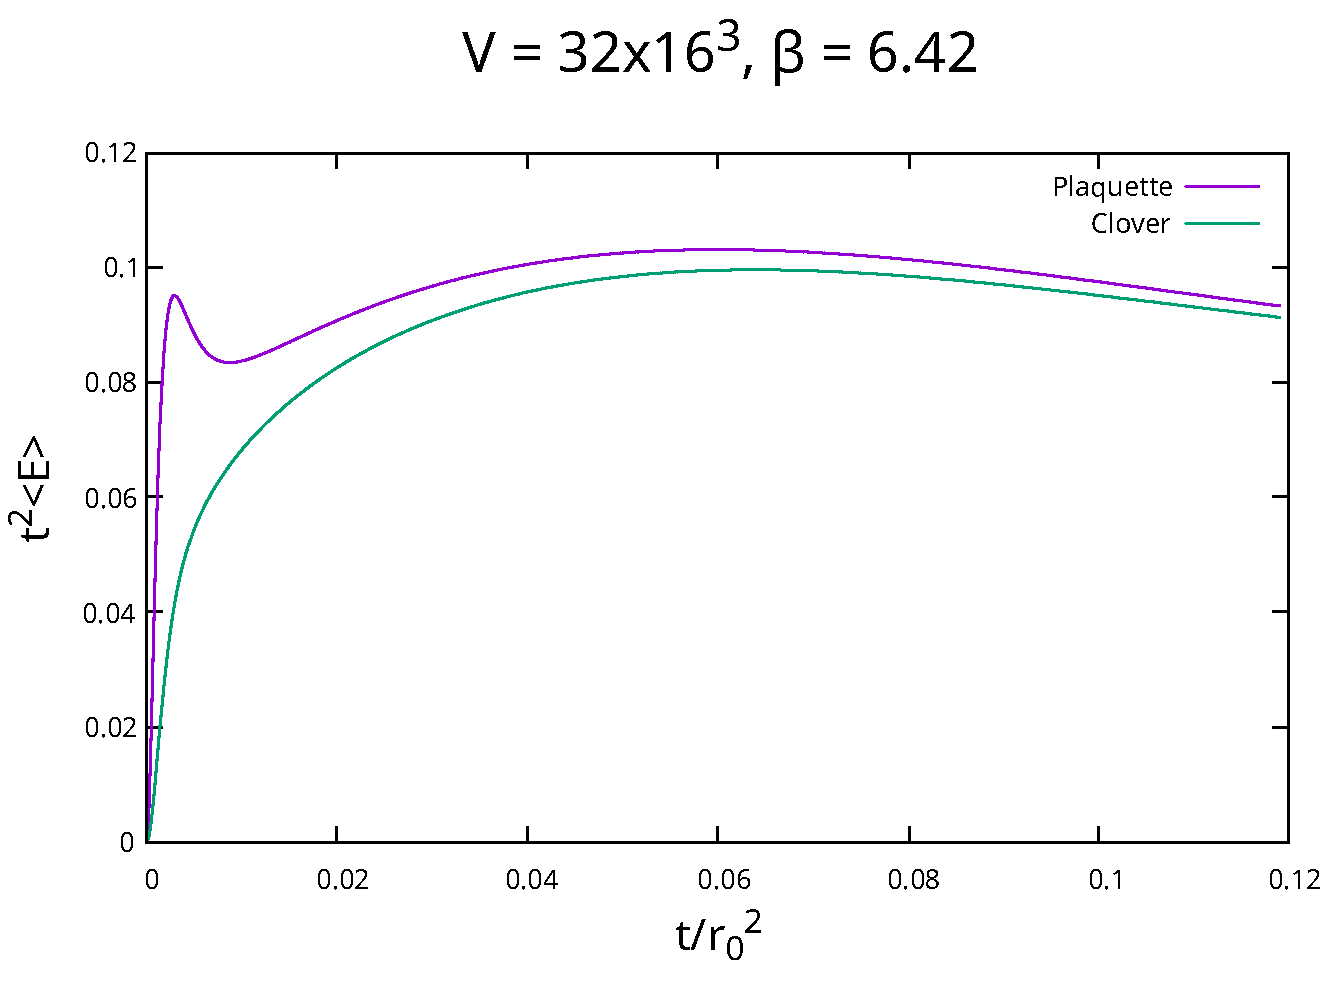
\includegraphics[scale=0.5]{WF_32x16.pdf}
    \caption{Simulation at $\beta = 6.42$ that corresponds to $a = 0.0498$ fm. With this volume finite size effects are strong. The integration scheme is done with RK3.}
\end{figure}



\section{Dynamical quarks}
Dirac matrix 
\begin{equation}
    D_{x,y;\alpha\beta}^{ab} = (m_0 + 4)\delta_{\alpha\beta}\delta^{ab}\delta_{x,y} - \frac{1}{2}\sum_{\mu = \pm 1}^{\pm 4}\left(\mathds{1} - \gamma_{\mu} \right)_{\alpha\beta}U^{ab}_{x,\mu}\delta_{x+\hat{\mu},y},
\end{equation}
where we define
\begin{equation}
    \gamma_{-\mu} = -\gamma_{\mu}, \ \ \ \mu = 1,2,3,4 .
\end{equation}

The fermion action for QCD reads
\begin{equation}
    S_{F}[\psi,\bar{\psi},U] = \sum_{f = 1}^{N_f} \sum_{x,y} \bar{\psi}^{(f)}_x D^{(f)}_{x,y} \psi^{(f)}_{y} .
\end{equation}

One usually computes the action of the Dirac operator on a vector $D\phi$
\begin{equation}
    D_{x,y;\alpha\beta}^{ab}\phi_{y,\beta}^{b} = (m_0+4)\phi_{x,\alpha}^{a} - \frac{1}{2}\sum_{\mu = \pm 1}^{\pm 4}\left(\mathds{1} - \gamma_{\mu} \right)_{\alpha\beta}U^{ab}_{x,\mu}\phi_{x+\hat{\mu},\beta}^{b}
\end{equation}

and $D^{\dagger}\phi$
\begin{equation}
    (D^{\dagger})_{x,y;\alpha\beta}^{ab}\phi_{y,\beta}^{b} = (m_0+4)\phi_{x,\alpha}^{a} - \frac{1}{2}\sum_{\mu = \pm 1}^{\pm 4}\left(\mathds{1} - \gamma_{\mu} \right)_{\alpha\beta}(U^{\dagger})^{ab}_{x-\hat{\mu},\mu}\phi_{x-\hat{\mu},\beta}^{b}
\end{equation}

\subsection{Hybrid Monte Carlo}
In the Hybrid Monte Carlo method an auxiliary field $P\in\su{3}$ is created and a Hamiltonian is defined as
 \begin{equation}
     H = \frac{1}{2}P^2 + S[U,\phi]
 \end{equation}
 where 
 \begin{equation}
     S[U,\phi] = S_G[U]-\phi^{\dagger}(DD^{\dagger})^{-1}\phi
 \end{equation}
 and
 \begin{equation}
     P^2 = \sum_{x,\mu} P_{x,\mu}^2 = -\frac{1}{2}\sum_{x,\mu} \tr(P_{x,\mu}^2)
 \end{equation}

\subsection{Leapfrog}
    \begin{enumerate}
        \item Generate the pseudofermion field $\phi = D\chi$, where $\chi$ is distributed according to $\exp(-\chi^{\dagger}\chi)$.
        \item Given a gauge configuration $[U]_0$ generate $[P]_0 \in \su{3}$ according to the Gaussian distribution $\exp(\tr[P^2])$.
        \item Initial step
            \begin{equation}
                P_{1/2} = P_0 - \frac{\epsilon}{2}F[U_0,\phi].
            \end{equation}
        \item Intermediate steps
        For $k = 1, \dots, n - 1 $:
            \begin{equation}
                U_{k} =  \exp\left( \epsilon P_{k-\frac{1}{2}}\right)U_{k-1} , \ \ \ P_{k+\frac{1}{2}} = P_{k-\frac{1}{2}} - \epsilon F[U_k,\phi]
            \end{equation}
        \item Final step
            \begin{equation}
                U_{n} =  \exp\left( \epsilon P_{n-\frac{1}{2}}\right)U_{n-1} , \ \ \ P_{n} = P_{n-\frac{1}{2}} - \frac{\epsilon}{2} F[U_n,\phi]
            \end{equation}
        \item Monte Carlo step. Accept/reject the configuration at the end of the trajectory with probability
            \begin{equation}
                \min\{1,\exp{\left(-\Delta H\right)}\}.
            \end{equation}
            where 
            \begin{equation}
                \Delta H = -\tr(P'^2) + \tr(P^2) + S_G[U'] - S_G[U] + \phi^{\dagger}\left( (D'D'^{\dagger})^{-1} - (DD^{\dagger})^{-1} \right)\phi
            \end{equation}
    \end{enumerate}

\begin{equation}
    F[U,\phi] = \sum_{a = 1}^8 T^i \nabla^{(i)} \left(S_G[U] + \phi^{\dagger}(DD^{\dagger})^{-1}\phi \right) \in \su{3}
\end{equation}

We define the auxiliary fields
\begin{equation}
    \psi = \left(DD^{\dagger}\right)^{-1}\phi, \ \ \ \chi = D^{\dagger} \psi .
\end{equation}

The force
\begin{eqnarray}
    \frac{\partial}{\partial \omega^i_{x,\mu}}\phi^{\dagger}\left( DD^{\dagger}\right)^{-1}\phi & = & -\phi^{\dagger}\left( DD^{\dagger}\right)^{-1} \frac{\partial DD^{\dagger}}{\partial \omega^i(x)} \left( DD^{\dagger}\right)^{-1} \phi \\
    & = & -\phi^{\dagger}\left[\left( DD^{\dagger}\right)^{-1}\left( \frac{\partial D}{\partial \omega^i_{x,\mu}}D^{\dagger}+D\frac{\partial D^{\dagger}}{\partial \omega^i_{x,\mu}}\right) \left( DD^{\dagger}\right)^{-1} \right]\phi \\
    & = & -2\re\left(\psi^{\dagger}\frac{\partial D}{\partial \omega^i_{x,\mu}}\chi \right)
\end{eqnarray}

with
\begin{eqnarray}
    \frac{\partial D_{y,z}\chi_z}{\partial \omega_{x,\mu}^i} & = & -\delta_{x,y}\frac{\mathds{1}-\gamma_{\mu}}{2}T^iU_{x,\mu}\chi_{x+\hat{\mu}}+\delta_{x+\hat{\mu},y}\frac{\mathds{1}+\gamma_{\mu}}{2}U^{\dagger}_{k,\mu}T^i\chi_{x}
\end{eqnarray}

The fermionic part of the force
\begin{eqnarray}
    \left(F_{\text{f}}\right)^i_{x,\mu} & = & -2\re\left\{-\left[T^i\right]^{ab}U_{x,\mu}^{bc} \left(\frac{1-\gamma_{\mu}}{2}\right)_{\alpha\beta} \chi_{x+\hat{\mu},\beta}^c \left(\psi^{a}_{x,\alpha}\right)^*\right\} \\
     &  & -2\re \left\{ (U_{x,\mu}^{\dagger})^{ab}[T^i]^{bc}\left( \frac{1+\gamma_{\mu}}{2}\right)_{\alpha\beta} \chi_{x,\beta}^{c} (\psi_{x+\hat{\mu},\alpha}^a)^* \right \} \\
     & = & -2\re \left\{-\left[T^i\right]^{ab}U_{x,\mu}^{bc} \left(\frac{1-\gamma_{\mu}}{2}\right)_{\alpha\beta} \left(\chi_{x+\hat{\mu},\beta}\otimes \psi^{\dagger}_{x,\alpha} \right)^{ca} \right\} \\
     &  & -2\re \left\{ (U_{x,\mu}^{\dagger})^{ab}[T^i]^{bc}\left(\frac{1+\gamma_{\mu}}{2}\right)_{\alpha\beta} \left(\chi_{x,\beta}\otimes \psi_{x+\hat{\mu},\alpha}\right)^{ca} \right \} \\
     & = & -2\re\tr\left\{-T^iU_{x,\mu} \left(\frac{1-\gamma_{\mu}}{2}\right)_{\alpha\beta} \left(\chi_{x+\hat{\mu},\beta}\otimes \psi^{\dagger}_{x,\alpha}\right) \right\} \\
     &  & -2\re \tr \left\{ U_{x,\mu}^{\dagger}T^i\left(\frac{1+\gamma_{\mu}}{2}\right)_{\alpha\beta} \left(\chi_{x,\beta}\otimes \psi^{\dagger}_{x+\hat{\mu},\alpha}\right) \right \} 
\end{eqnarray}
Then
\begin{equation}
    \left(F_{\text{f}}\right)_{x,\mu} = \left\{-U_{x,\mu} \left(\frac{1-\gamma_{\mu}}{2}\right)_{\alpha\beta} \chi_{x+\hat{\mu},\beta}\otimes\psi^{\dagger}_{x,\alpha} + \left(\frac{1+\gamma_{\mu}}{2}\right)_{\alpha\beta}       \chi_{x,\beta}\otimes \psi^{\dagger}_{x+\hat{\mu},\alpha}U_{x,\mu}^{\dagger} \right\}_{\text{TA}}
\end{equation}

\begin{figure}
    \centering
    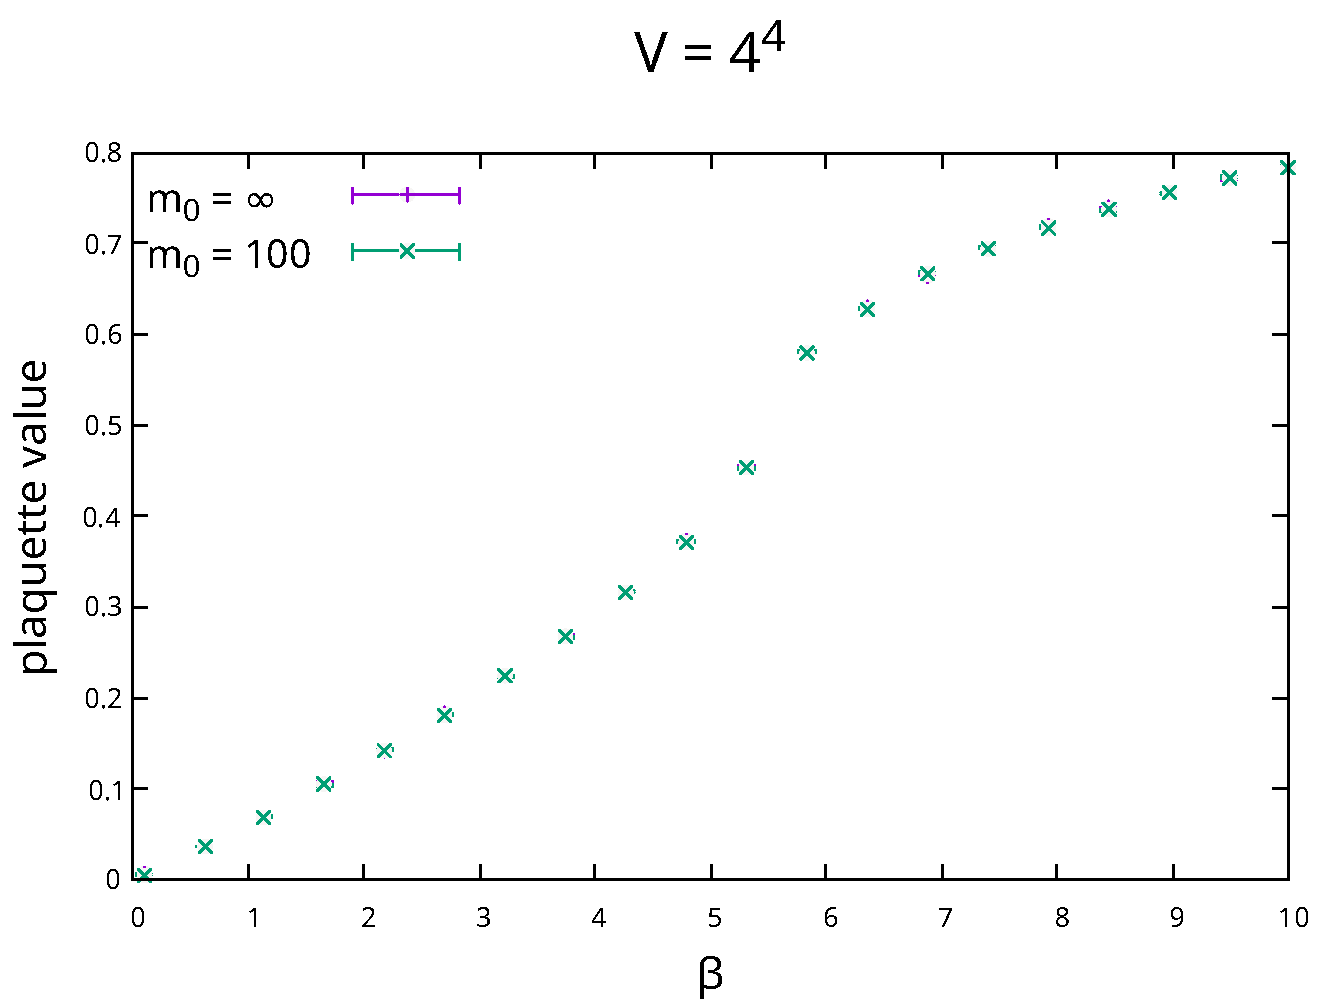
\includegraphics[scale=0.5]{plq.pdf}
    \caption{Plaquette value of the pure gauge SU(3) theory with $m_0=\infty$ using heatbath and with dynamical quarks at $m_0 = 100$ with hybrid Monte Carlo.}
\end{figure}


\section{Topological charge density}

The topological charge $Q[U]$ of a configuration $[U]$ is defined as the sum over the lattice of the topological charge density $q(x)$ 
\begin{equation}
    q(x) = -\frac{1}{32\pi^2}\varepsilon_{\mu\nu\rho\sigma} \text{Tr} \left\{ F_{\mu\nu}(x)F_{\rho\sigma}(x)\right\}.
\end{equation}
On the lattice, we can define the topological charge with the clover or plaquette definitions of $F_{x,\mu\nu}$. Using the symmetries of the clover definition we can reduce the number of sums to be computed. First, we note that only 24 elements of the Levi-Civita symbol are non-zero. We also note that
\begin{eqnarray}
    \varepsilon_{\mu\nu\rho\sigma} \text{Tr} \left\{ F^{\text{clover}}_{x,\mu\nu}F^{\text{clover}}_{x,\rho\sigma}\right\} & = & \varepsilon_{\nu\mu\rho\sigma} \text{Tr} \left\{ F^{\text{clover}}_{x,\nu\mu}F^{\text{clover}}_{x,\rho\sigma}\right\} \\
    \varepsilon_{\mu\nu\rho\sigma} \text{Tr} \left\{ F^{\text{clover}}_{x,\mu\nu}F^{\text{clover}}_{x,\rho\sigma}\right\} & = & \varepsilon_{\mu\nu\sigma\rho} \text{Tr} \left\{ F^{\text{clover}}_{x,\mu\nu}F^{\text{clover}}_{x,\sigma\rho}\right\} \\
    \varepsilon_{\mu\nu\rho\sigma} \text{Tr} \left\{ F^{\text{clover}}_{x,\mu\nu}F^{\text{clover}}_{x,\rho\sigma}\right\} & = & \varepsilon_{\rho\sigma\mu\nu} \text{Tr} \left\{F^{\text{clover}}_{x,\rho\sigma}F^{\text{clover}}_{x,\mu\nu}\right\}
\end{eqnarray} 
This reduces the number of effective sums by a factor of 8. From the original 24 sums we only need to perform 3.

Using $Q$ instead of $F$ we arrive at
\begin{equation}
    \text{Tr}\left\{F^{\text{clover}}_{x,\mu\nu}F^{\text{clover}}_{x,\rho\sigma}\right\} =\frac{1}{2^5} \re\text{Tr}\left\{Q_{x,\mu\nu}\left[Q_{x,\rho\sigma}-Q_{x,\rho\sigma}^{\dagger}\right]\right\}
\end{equation}
We choose the 3 independent permutations of $\varepsilon_{\mu\nu\rho\sigma}$ to be in the indices $[1,2,3,4]$, $[1,3,2,4]$ and $[1,4,2,3]$. Therefore,
\begin{equation}
    q^{\text{clover}}_x = -\frac{1}{128 \pi^2} \sum_{[\mu\nu\rho\sigma] \in\{ [1234], [1324], [1423]\}}
              \varepsilon_{\mu\nu\rho\sigma}\re\tr\left(Q_{x,\mu\nu}\left[Q_{x,\rho\sigma}-Q_{x,\rho\sigma}^{\dagger}\right]\right) 
\end{equation}


\section{Acknowledgements}
The author thanks Dr.\ Wolfgang Bietenholz for funding (in the form of meals) this research. Thanks to Dr.\ Urs Gerber for providing a recipe for implementing the heatbath algorithm for the U(1) gauge theory at an early stage of this research. Thanks to MSc.\ Jaime Fabián Nieto Castellanos for his help in the implementation of the Hybrid Monte Carlo algorithm in the Schwinger model. I want to thank Ariana Grande, The Weeknd and Polyphia for giving the right inspiration while working on this paper. Without their music I could have easily gone crazy.

\begin{thebibliography}{99}

\bibitem{gattringer} C.\ Gattringer and C.B.\ Lang, \emph{Quantum Chromodynamics on the Lattice: An Introductory Presentation},  Lect.\ Notes Phys.\ 788 (Springer, Berlin Heidelberg 2010).

\bibitem{Metropolis} N.\ Metropolis {\it et al.},
\emph{Equation of State Calculations by Fast Computing Machines},
J.\ Chem.\ Phys.\ {\bf 21} (1953) 1087.

\bibitem{Glauber} R.J.\ Glauber,
  \emph{Time-Dependent Statistics of the Ising Model},
  J.\ Math.\ Phys.\ {\bf 4} (1963) 294.
  
\bibitem{Gerber} U.\ Gerber,
  \emph{Heatbath Algorithm for the 2d U(1) Model}.
  Informal Notes. Universidad Nacional Autónoma de México, 2015.  
  
  \bibitem{creutz1980} M. Creutz, \emph{Monte Carlo Study of the Quantized SU(2) Gauge Theory.} Phys.\ Rev.\ D {\bf 21} (1980) 2308-2315.

\bibitem{cabbibo1982} N. Cabbibo, E. Marinari, \emph{A New Method for Updating SU(N) Matrices in Computer Simulations of Gauge Theories}, Phys.\ Lett.\ B {\bf 119} (1982) 387-390.

\bibitem{kennedy1985} A.D.\ Kennedy, B.J.\ Pendleton, \emph{Improved Heatbath Method for Monte Carlo Calculations in Lattice Gauge Theories}, Phys.\ Lett.\ {\bf 156B} (1985) 393-399.

\bibitem{luscher2014} M.\ L\"uscher, \emph{Properties and uses of the Wilson flow in lattice QCD}, 2014.

\bibitem{2flqcd} J.A.\ García-Hernández, Lattice QCD code: \url{https://github.com/JoseAntonioLattice/2FLQCD.git}
\end{thebibliography}

\end{document}
